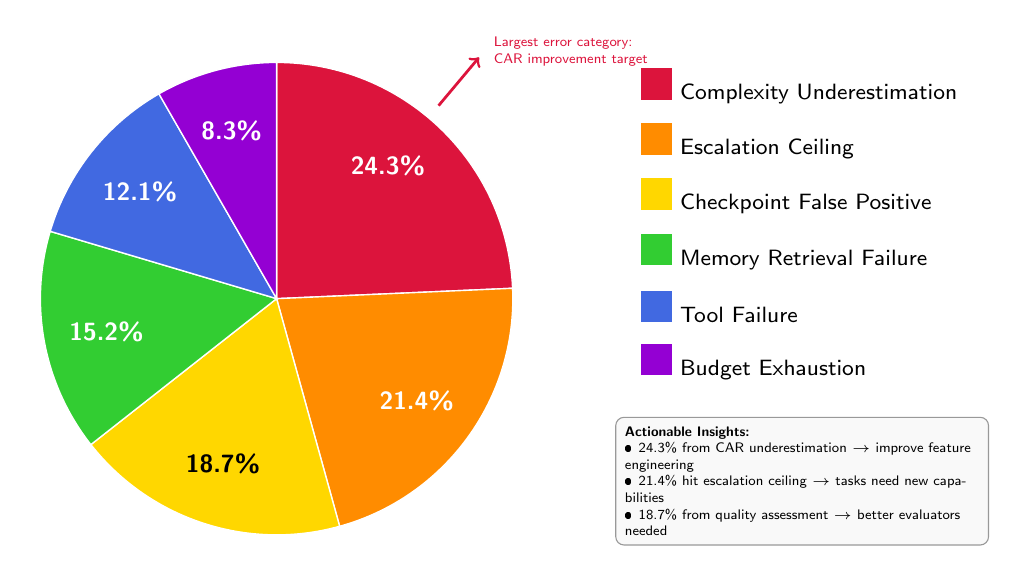
\begin{tikzpicture}[
	slice/.style={line width=0.5pt, draw=white}
	]
	% Title
%	\node[font=\sffamily\small, color=gray] at (0,4.5) {(Distribution of failure cases)};
	
	% Define colors
	\definecolor{cu}{RGB}{220,20,60}      % Crimson - Complexity Underestimation
	\definecolor{ec}{RGB}{255,140,0}      % Dark Orange - Escalation Ceiling
	\definecolor{cfp}{RGB}{255,215,0}     % Gold - Checkpoint False Positive
	\definecolor{mrf}{RGB}{50,205,50}     % Lime Green - Memory Retrieval Failure
	\definecolor{tf}{RGB}{65,105,225}     % Royal Blue - Tool Failure
	\definecolor{be}{RGB}{148,0,211}      % Dark Violet - Budget Exhaustion
	
	% Draw pie slices
	% Starting from 90 degrees (top), going clockwise
	% Complexity Underestimation (24.3%) - 0 to 87.48
	\fill[cu, slice] (0,0) -- (90:3) arc (90:2.52:3) -- cycle;
	% Escalation Ceiling (21.4%) - 87.48 to 164.52
	\fill[ec, slice] (0,0) -- (2.52:3) arc (2.52:-74.52:3) -- cycle;
	% Checkpoint False Positive (18.7%) - 164.52 to 231.84
	\fill[cfp, slice] (0,0) -- (-74.52:3) arc (-74.52:-141.84:3) -- cycle;
	% Memory Retrieval Failure (15.2%) - 231.84 to 286.56
	\fill[mrf, slice] (0,0) -- (-141.84:3) arc (-141.84:-196.56:3) -- cycle;
	% Tool Failure (12.1%) - 286.56 to 330.12
	\fill[tf, slice] (0,0) -- (-196.56:3) arc (-196.56:-240.12:3) -- cycle;
	% Budget Exhaustion (8.3%) - 330.12 to 360
	\fill[be, slice] (0,0) -- (-240.12:3) arc (-240.12:-270:3) -- cycle;
	
	% Labels with percentages
	\node[font=\sffamily\small\bfseries, color=white] at (50:2.2) {24.3\%};
	\node[font=\sffamily\small\bfseries, color=white] at (-36:2.2) {21.4\%};
	\node[font=\sffamily\small\bfseries, color=black] at (-108:2.2) {18.7\%};
	\node[font=\sffamily\small\bfseries, color=white] at (-169:2.2) {15.2\%};
	\node[font=\sffamily\small\bfseries, color=white] at (-218:2.2) {12.1\%};
	\node[font=\sffamily\small\bfseries, color=white] at (-255:2.2) {8.3\%};
	
	% Legend
	\node[font=\sffamily\footnotesize, anchor=west] at (4.5,2.7) {\textcolor{cu}{\rule{0.4cm}{0.4cm}} Complexity Underestimation};
	\node[font=\sffamily\footnotesize, anchor=west] at (4.5,2.0) {\textcolor{ec}{\rule{0.4cm}{0.4cm}} Escalation Ceiling};
	\node[font=\sffamily\footnotesize, anchor=west] at (4.5,1.3) {\textcolor{cfp}{\rule{0.4cm}{0.4cm}} Checkpoint False Positive};
	\node[font=\sffamily\footnotesize, anchor=west] at (4.5,0.6) {\textcolor{mrf}{\rule{0.4cm}{0.4cm}} Memory Retrieval Failure};
	\node[font=\sffamily\footnotesize, anchor=west] at (4.5,-0.1) {\textcolor{tf}{\rule{0.4cm}{0.4cm}} Tool Failure};
	\node[font=\sffamily\footnotesize, anchor=west] at (4.5,-0.8) {\textcolor{be}{\rule{0.4cm}{0.4cm}} Budget Exhaustion};
	
	% Exploded slice indicator for largest category
	\draw[->, line width=1pt, color=cu] (50:3.2) -- (50:4);
	\node[font=\sffamily\tiny, color=cu, anchor=west, text width=3cm] at (50:4.1) {Largest error category:\\CAR improvement target};
	
	% Insight box
	\node[draw=black!40, fill=gray!5, rounded corners=3pt, font=\sffamily\tiny, text width=4.5cm, align=left, anchor=north west] at (4.3,-1.5) {
		\textbf{Actionable Insights:}\\
		\textbullet\ 24.3\% from CAR underestimation $\rightarrow$ improve feature engineering\\
		\textbullet\ 21.4\% hit escalation ceiling $\rightarrow$ tasks need new capabilities\\
		\textbullet\ 18.7\% from quality assessment $\rightarrow$ better evaluators needed
	};
\end{tikzpicture}